\FloatBarrier
\subsection{Filter cavities}\label{app:filtercavities}

The necessity of filter cavities for a broadband quantum noise reduction with a squeezed state of light was described in Secs.~\ref{subsec:qnft}, \ref{subsec:QNRsqz}, and \ref{subsec:SQZforGWD}. In the following sections, the technical requirements for these optical filters are discussed. An important point is the required baseline length of these filter cavities in view of their optical round-trip loss (Sec.~\ref{subsec:FClength}). The tolerances of the determined design parameters will be discussed in Sec.~\ref{subsec:robustparam}.   Furthermore, in Sec.~\ref{subsec:fcscattering} the optical layout with regard to the round-trip loss that will be mainly caused by scattering by the mirror surface defects is treated. Finally, the degradation of the squeezing level due to noise couplings (e.g.\ displacement noise in the filter cavities) will be analysed in Sec.~\ref{sec:noise}, leading to further estimates for the requirements.


\FloatBarrier
\subsubsection{Restrictions for the baseline length of the filter cavity}\label{subsec:FClength}


In this Section we start with a description of the influence of optical round-trip loss on the filter cavities performance in dependence of their baseline length and half-bandwidth. The required half-bandwidth $\gamma_{\rm fc}$ and detuning
$\Phi_{\rm fc}$
(note that we will define them as angular
frequencies) of the filter cavities giving the optimal frequency-dependent squeezing angle are determined by the interferometer
configuration and its induced phase-space rotation of light fields
entering the interferometers output port. The determination of these values is presented in Sec.~\ref{sec:detfcparams} in detail.

Generally, any round-trip loss will degrade the squeezing level at
sideband frequencies being resonant in the filter cavity. For a
given power round-trip loss $l^2_{\rm rt,fc}$ (mainly caused by
scattering)  the resulting loss in reflection of the filter cavity
increases with a decreasing baseline length $L_{\rm fc}$ of the
filter. As well, for a certain length  $L_{\rm fc}$ and a certain
round-trip loss $l^2_{\rm rt,fc}$ the loss imposed on the squeezed
field increases with a decreasing half-bandwidth $\gamma_{\rm fc}$
that needs to be realized. Starting from the expression for the
half-bandwidth of a lossy cavity
\begin{equation} \gamma_{\rm fc} = \frac{c}{2 L_{fc}}
\arccos\left(1-\frac{(1-\rho_{\rm c}\sqrt{1- l^2_{\rm
rt,fc}})^2}{2\rho_{\rm c}\sqrt{1- l^2_{\rm
rt,fc}}}\right)\,\label{eq:gamma}
\end{equation}
one can derive the filter cavity's coupling mirror power reflectance
$R_{\rm c}=\rho_{\rm c}^2$ that is required to achieve the
targeted half-bandwidth. One obtains
\begin{equation}
\rho_{\rm c} = \frac{1}{\sqrt{1- l^2_{\rm
rt,fc}}}\left[2-\cos(\mathcal{F}^\prime) -
\sqrt{\cos^2(\mathcal{F}^\prime)-4 \cos(\mathcal{F}^\prime)+3}
\right]\label{eq:rc}
\end{equation}
with
\begin{equation}
\mathcal{F}^\prime =  \frac{2 \gamma_{\rm fc} L_{\rm fc}}{c} =
\frac{\gamma_{\rm fc}}{{\rm FSR_{fc}}}
=\frac{\pi}{\mathcal{F}_{\rm fc}}\,.
\end{equation}

\begin{figure}
\centering
\includegraphics[scale = 1.2]{./Sec_Optics/FCsgammaAI75ppm.pdf}
\caption{Filter cavity properties in dependence of its half-bandwidth $\gamma_{\rm fc}$.  a) the remaining detectable squeezing level in reflection of the filter cavity and b) its reflectance at the frequency $\Omega =  \Phi_{\rm fc}L_{\rm fc}/c$. In c) the value for $L_{\rm cc}$ is shown according to Eq.~(\ref{eq:lcc}).  Curve d) shows the finesse and e) the coupling mirror reflectance $R_{\rm c}$ given by Eq.~(\ref{eq:rc}). For all traces a filter cavity length $L_{\rm fc}=10\,{\rm km}$ and a round-trip loss $l_{\rm rt,fc}^2=75\,{\rm ppm}$ was assumed. An initial pure 10\,dB squeezed state was considered. It can be seen that the impact of the round-trip loss becomes significant for $\gamma_{\rm fc}<2\pi\cdot10\,{\rm Hz}$.} \label{fig:gamma}
\end{figure}

Graph e) in Fig.~\ref{fig:gamma} shows the value for $R_{\rm
c}=\rho_{\rm c}^2$ according to Eq.~(\ref{eq:rc}). In the
underlying calculations the baseline length $L_{\rm fc}$ and the
round-trip loss $l_{\rm rt,fc}^2$ were considered with 10\,km and
75\,ppm, respectively.  The tuning of the filter cavity was
exemplary set to $\Phi_{\rm fc}=\gamma_{\rm fc}L_{\rm fc}/c$. It
can be seen, that for small half-bandwidths $\gamma_{\rm fc}$ the
reflectance  $R_{\rm c}$ comes close to unity.  Correspondingly,
the resulting finesse rises as shown in Graph d). It can be seen
from Eq.~(\ref{eq:rc}) that there are two fundamental restrictions
for the choice of the filter cavity length. First, for great
values of the finesse (i.e.\ for small half-bandwidths) we obtain
\begin{equation}
\lim_{\gamma_{\rm fc} \to 0} \rho_{\rm c} = \frac{1}{\sqrt{1-l_{\rm rt,fc}^2}}> 1
\end{equation}
which does not represent a physical solution. Thus, there must
exist a value $L_{\rm min}$ such that for $L_{\rm min} < L_{\rm
fc}$ we always have $\rho_{\rm c}<1$. The expression for $L_{\rm
min}$ can be derived to
\begin{equation}
L_{\rm{min}} =
\frac{c}{2\gamma_{\rm{fc}}}\arccos\left[2-\frac{2-l_{\rm{rt,fc}}^2}{2\sqrt{1-l_{\rm{rt,fc}}^2}}\right]\,.
\end{equation}

Second, for $L_{\rm fc} < L_{\rm cc}$ we obtain $\rho_{\rm
c}>\sqrt{1-l_{\rm rt,fc}^2}$ and the filter cavity becomes
under-coupled. But even in the most general case, the
interferometer represents an over-coupled cavity. Hence, an
under-coupled filter cavity with $L_{\rm fc} < L_{\rm cc}$ can not
provide the phase-space rotation required for the generation of
the optimal squeezing angle.

To keep  $\rho_{\rm c}<\sqrt{1-l_{\rm rt,fc}^2}$ the filter cavity length needs to be
\begin{equation}
L_{\rm fc} > L_{\rm cc} =
\frac{c}{2\gamma_{\rm{fc}}}\arccos\left[2-\frac{1+(1-l_{\rm
rt,fc}^2)^2}{2(1-l_{\rm rt,fc}^2)}\right]\label{eq:lcc}
\end{equation}
Note that for $L_{\rm fc}=L_{\rm cc}$ the filter cavity is
critically coupled (impedance matched) and the loss in its
reflection is maximum. Therefore, to preserve the squeezing in
reflection of the filter cavities its length should be chosen with
$L_{\rm fc} \gg L_{\rm cc}$. This fact becomes obvious when
looking at graph a) and b) of Fig.~\ref{fig:gamma}. They show the
squeezing level in reflection of the filter cavity and the according reflectance of the filter cavity at its resonance frequency, respectively. At small half-bandwidths the
value for $L_{\rm cc}$ (graph c)) is of the order of the filter
cavity's baseline length $L_{\rm fc}=10\,{\rm km}$ and hence the reflectance
and accordingly the remaining squeezing level are considerably
reduced.

\begin{figure}
\centering
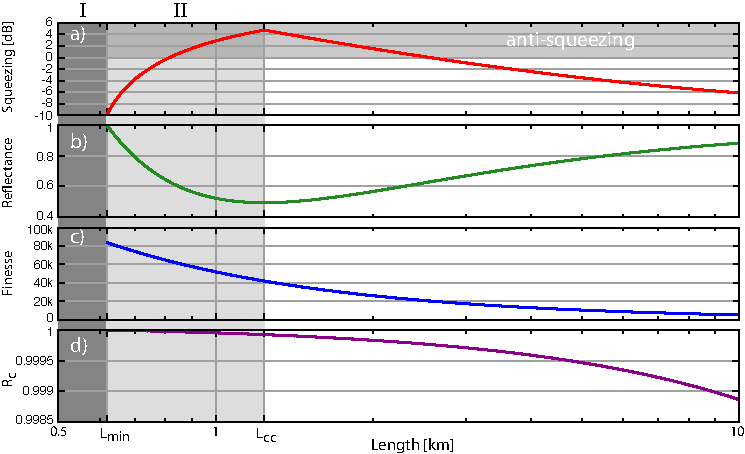
\includegraphics [scale = 1.1]{./Sec_Optics/FCslength75ppmAI.pdf}
\caption{The figure shows the filter cavity performance in dependence of its baseline length $L_{\rm fc}$. Graph~a) shows the remaining squeezing level in reflection of the filter cavity at its resonance frequency. Graph~b) shows the according  reflectance of the filter cavity. Graph~c) and d) show the filter cavity finesse and coupling mirror reflectance $R_{\rm c}$, respectively. The two grey shaded areas in the left highlight the region where $L_{\rm fc}<L_{\rm cc}$ (area II) and where $L_{\rm fc}<L_{\rm min}$ (area I). In the considered example ($\gamma_{\rm fc} =2\pi\cdot1.4\,{\rm Hz}$, $\Phi_{\rm fc_1}= 2\pi\cdot6.6\,{\rm Hz}\cdot L_{\rm fc_1}/c$,  $l^2_{\rm rt,fc}=75\,{\rm ppm}$) the critical length $L_{\rm cc}$ is about 1239\,m. The top grey shaded area in graph a) highlights the anti-squeezed region. Due to the unbalanced loss for upper and lower squeezing sidebands in the detuned filter cavity, for high resulting loss (i.e.\ for a cavity reflectance much smaller than one) the detected noise can be even enhanced when compared to the vacuum noise (refer to Fig.~\ref{fig:sqzphspic}). In the considered example the detected noise is already enhanced (anti-squuezed) for filter cavity baseline lengths smaller than approximately 2.5\,km.}
\label{fig:length}
\end{figure}



\begin{figure}
\centering
Fig.\ to be added%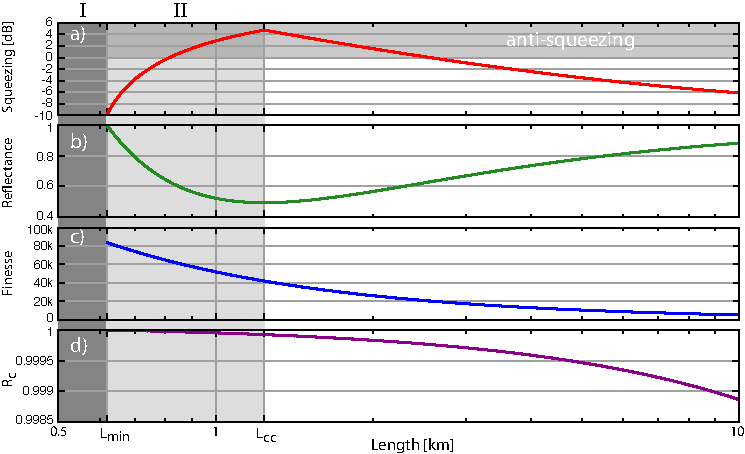
\includegraphics [scale = 1.1]{./Sec_Optics/FCslength75ppmAI.pdf}
\caption{Some nice phasors showing the effect of unbalanced loss\dots}
\label{fig:sqzphspic}
\end{figure}


In Fig.~\ref{fig:length}  the filter cavity performance is shown
depending on its baseline length $L_{\rm fc}$. In the
corresponding calculations we assumed the target half-bandwidth
with ${\gamma_{\rm fc} = 2\pi\cdot1.4\,{\rm Hz}}$ and the target detuning with
${\Phi_{\rm fc_1}= 2\pi\cdot 6.6\,{\rm Hz}\cdot L_{\rm fc_1}/c}$.
Note, that these values are approximately the requirements for one of the filter
cavities that needs to be realised in the ET-LF
detector~\cite{Hild2010a}. Again, the round-trip loss was
considered of 75\,ppm and the initial squeezing level of 10\,dB.  Graph a)
demonstrates, that even with a filter cavity length of 10\,km the
amount of squeezing  is already reduced by a factor of about
4\,dB. For lengths smaller than about 2.5\,km the unbalanced loss for upper and lower squeezing sidebands results in a noise enhancement (anti-squeezing) when compared to vacuum noise in reflection of the filter cavity.  At the crtical length $L_{\rm fc} = L_{\rm
cc}\approx1239\,\rm m$ this enhancement becomes maximum and corresponds to about 5\,dB anti-squeezing. For lengths smaller than $L_{\rm cc}$  the noise level drops and squeezing can be achieved again (grey shaded area~II) until it reaches at $L_{\rm fc} =
L_{\min}$ the initial level of 10\,dB. However, in this region the
filter is under-coupled and does not yield the required
phase-space rotation of the squeezed field. This can be understood
when considering the extreme case for $L_{\rm fc} = L_{\min}$.
Here, $R_{\rm c}$ is equal to one and  the filter cavity can be
replaced by  an ordinary mirror that has no frequency dependence.
Again, it can be deduced that a filter cavity length  $L_{\rm fc}
\gg L_{\rm cc}$ needs to be realised in order to preserve the
squeezing. In addition, the high finesse of a short cavity might
pose a problem for the lock acquisition in the environment of a gravitational-wave detector where the optics
needs to be suspended.

So far in Figs.~\ref{fig:gamma} and~\ref{fig:length} the squeezing level was shown in reflection of the considered filter cavities at its resonance frequency. Here the  (frequency-dependent) imposed loss is maximum. Now, for  exemplification
Fig.~\ref{fig:sqz} shows squeezing spectra obtained after the
reflection at two subsequent filter cavities FC$_1$ and FC$_2$.
The considered  half-bandwidths and tunings of these filters are
those needed for the ET-LF detector. The length of the cavities
were considered with  $L_{\rm fc_1}=L_{\rm fc_2}=2\,{\rm km}$ (red
curve), $L_{\rm fc_1}=L_{\rm fc_2}=5\,{\rm km}$ (blue curve) and
$L_{\rm fc_1}=L_{\rm fc_2}=10\,{\rm km}$ (green curve),
respectively.


The calculations and exemplary filter properties considered within
this Section imply that in 3rd generation GWADS
detectors such as the Einstein Telescope, where filter cavities with half-bandwidths
in the range of ${\gamma_\text{fc}\approx 2\pi\cdot1- 2\pi\cdot5\,\mathrm{Hz}}$ will be
required, the baseline length of these filters needs to be in the
order of a few kilometers. This contrasts to the results presented
in \cite{Khalili2009} for the Advanced LIGO
detector. As for the Advanced LIGO configuration filter cavities with
half-bandwidths in the order of ${2\pi\cdot50- 2\pi\cdot200\,{\rm Hz}}$ will be required, a
considerable sensitivity increase by the injection of frequency-dependent squeezed light can already be achieved if filter
cavities with lengths in the order of 100\,m are utilised. Certainly,
our exemplary calculations are based on a conservative assumption
of 75\,ppm for the round-trip loss of the filter cavities, but
even if optimistic values of $l_{\rm rt,fc}^2=20\,\mathrm{ppm}$ are
considered, the corresponding values for the critical lengths will
be $L_{\rm cc, fc_1} = 330\,{\rm m}$ and  $L_{\rm cc, fc_2} =
84\,{\rm m}$, respectively. As shown in Figs.~\ref{fig:gamma}
and \ref{fig:length} the respective length $L_{\rm fc}$ should be
at least 10 times greater than $L_{\rm cc}$.   I.e.\ for the ET-LF detector the  length of the two required filter cavities should be 10\,km. In contrast, it can be shown that for the ET-HF detector a filter with a length of about 500\,m is sufficient. This filter will be required for an optimisation of the squeezed quadrature in the radiation pressure noise dominated frequency band. However, in this frequency band other noise sources dominates the quantum noise. For that it is satisfactory to adapt the squeezing level to the level of these noise sources which will be possible with a comparatively short filter cavity.



The former investigation demonstrated that  the round-trip loss ultimately restricts the minimal allowed baseline length and consistently the performance of the filter cavities. As it is expected that the round-trip loss of the filters will be dominated by scattering at imperfect mirror surfaces, the optical layout needs to be designed such that the amount of scattering is as much as possible reduced. The scattering in different optical layouts is treated in Sec.~\ref{subsec:fcscattering}.

\begin{figure}
\centering
\includegraphics[scale = 1.2] {./Sec_Optics/ET-C-FiltersAI.pdf}
\caption{The figure shows the remaining squeezing level after subsequent reflection at two filter cavities FC$_1$ and FC$_2$. In graph~a) an initial pure 10\,dB squeezed state was considered and 75\,ppm round-trip loss in each cavity. Additionally, in graph~b)  optical loss of 9\,\% outside the filter cavities was considered. Thus, an initial pure 20\,dB squeezed state is necessary to achieve 10\,dB detectable squeezing. In both cases, three length of the cavities were considered. The green curves are obtained for $L_{\text{fc}_1}=L_{\text{fc}_2}=10\,\mathrm{km}$, the blue one for  $L_{\text{fc}_1}=L_{\text{fc}_2}=5\,\mathrm{km}$ and the red one for  $L_{\text{fc}_1}=L_{\text{fc}_2}=2\,\mathrm{km}$. The filter parameters are approximately those that are required for a broadband quantum noise reduction in the ET-LF detector, i.e.\ $\gamma_{\text{fc}_1}=2\pi\cdot1.4\,\mathrm{Hz}$, $\Phi_{\text{fc}_1}= 2\pi\cdot6.6\,\mathrm{Hz}\cdot L_{\text{fc}_1}/c$ and $\gamma_{\text{fc}_1}=2\pi\cdot5.7\,\mathrm{Hz}$, $\Phi_{\text{fc}_1}= -2\pi\cdot25.4\,\mathrm{Hz}\cdot L_{\text{fc}_1}/c$, respectively. Please note, that from this comparison it can be deduced, that the tolerable loss in the filters needs to be determined also in view of the injected anti-squeezing.}
\label{fig:sqz}
\end{figure}
\FloatBarrier
\subsubsection{Determination of the required filter parameters}\label{sec:detfcparams}

In publications by Purdue and Chen~\cite{PurduePRD66} and Harms \cite{HarmsPRD68} treating the frequency dependent squeezed light injection, some analytical expressions were derived showing first the need for filter cavities and second allow for a calculation of the required number,  bandwidth and tuning of filter cavities.
In these works the interferometer quantum noise transfer function was derived using the Caves-Schumacher two-photon formalism~\cite{Caves}. The interferometer quantum noise transfer function is then described by a $2\times 2$-matrix $\mathbf{T}$ (refer to Eq.~(3) in \cite{HarmsPRD68}).  From this matrix the required frequency-dependent squeezing angle $\lambda(\Omega)$ can be derived according to Eq.~(16) in \cite{HarmsPRD68}


\begin{equation}
\lambda(\Omega) = \arctan\left(-\frac{T_{11}\cos\zeta + T_{21}\sin\zeta}{T_{12}\cos\zeta + T_{22}\sin\zeta}\right)\,.\label{eq:lopt}
\end{equation}
Here, $\Omega$ is the angular sideband frequency and $\zeta$ the read-out angle. It was shown in \cite{PurduePRD66}, that with a combination of Fabry-Perot cavities the required frequency dependent angle $\lambda(\Omega)$ can be realized. It  has the form \cite{PurduePRD66}
\begin{equation}
\tan\lambda(\Omega) = \frac{\sum_{k=0}^{n} B_k\Omega^{2k}}{ \sum_{k=0}^{n} A_k\Omega^{2k}}\,, \text{with}\, \left|A_n+\mathrm{i}B_n\right|>0
\end{equation}
From the corresponding characteristic equation
\begin{equation}
\sum_{k=0}^{n} \left(A_k+\mathrm{i}B_k\right)\Omega^{2k}=0\label{eq:chareq}
\end{equation}
the required bandwidth and tuning of the filter cavities can be obtained. They are given by the $2n$ roots (in $n$ pairs with a positive imaginary part) of Eq.~(\ref{eq:chareq}).
However, these calculations are based on the assumption of a lossless main interferometer, an infinite small signal-recycling cavity length,  an expansion in powers of the light's angular frequency and the approximated expression for a cavity's half-bandwidth $\gamma=c\tau/(4L)$. Thus, in general they allow just for a precise estimation for the required parameters.
Furthermore it is demonstrated in Fig.~\ref{fig:phs-vs-loss}, that it is not sufficient to realize filter cavities having the bandwidth and tuning determined by Eq.~(\ref{eq:chareq}).   First, the impact of optical loss was considered. Therefore, the phase-space rotation in reflection of a cavity with a half-bandwidth $\gamma=2\pi\cdot1.44448\,\rm Hz$ and a tuning according  to $f_{\rm res} = 6.628\,\rm Hz$ is calculated for different values of the round-trip loss. The lenght was set to 10\,km. The results are shown in the left graph of Fig.~\ref{fig:phs-vs-loss}. It can be seen that the deviation of the phase-space rotation related to the lossless case increases with increasing optical loss. Similarly, the rotation in reflection depends on the baseline length of the cavity. This fact is shown in the right graph of Fig.~\ref{fig:phs-vs-loss}. Here, the round-trip loss was set to 75\,ppm for all cases.


 \begin{figure}
 \centering
   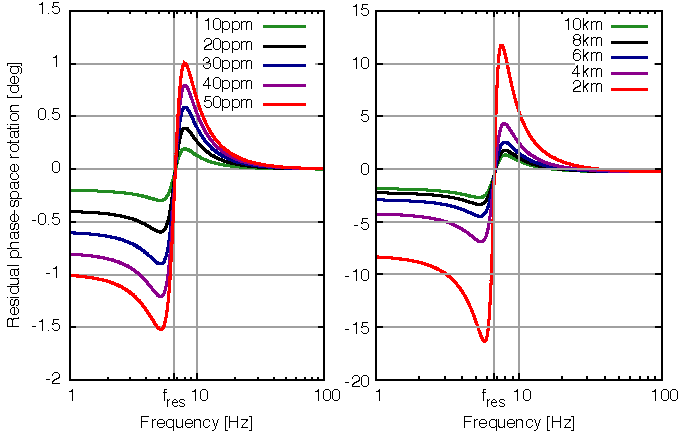
\includegraphics{./Sec_Optics/PhsRot-residualsAI.pdf}
   \caption{The figure demonstrates, that the phase-space rotation of a Fabry-Perot cavity is not only determined by its resonance frequency and bandwidth (here exemplary set to 6.628\,Hz and 1.44448\,Hz, respectively, for all cases), but also by its round-trip loss (left) and its baseline length (right).}
   \label{fig:phs-vs-loss}
   \end{figure}


Especially under consideration of optical intra-cavity round-trip loss and a finite baseline length of the filter cavities as well as the signal-recycling cavity,
there is no possibility to determine the optimal filter cavities parameters analytically. Thus, the parameters for the filter cavities were fitted with respect to the residual phase-space rotation of injected squeezed field. Fig.~\ref{fig:phs-fit-75ppm} compares the results for the parameters determined in accordance to Eq.~\ref{eq:chareq} (red curve) and those determined by the fit (black curve) for the ET-D LF detector. The corresponding filter cavity parameters are listed in Tab.~\ref{tab:fitanaparamsloss}

\begin{figure}
 \centering
   \includegraphics{./Sec_Optics/Fit_realparams.pdf}
   \caption{The figure shows the residual rotation of the injected squeezing, if the filter cavities are realized with parameters determined in accordance to Eq.~(\ref{eq:chareq}) (red curve) and those determined by  a fit (black curve). After fitting the parameters, the residual rotation is less than 0.2 deg.}
   \label{fig:phs-fit-75ppm}
   \end{figure}


\begin{table}[h]
\centering
\begin{tabular}{c|c|c}
\hline
\hline
 & tuning [Hz]  (fitted / analytical) & half-bandwidth [Hz] (fitted / analytical)\\
\hline
FC$_1$ &-25.4255 / -25.3592  & 5.76766 / 5.68148\\
FC$_2$ & 6.6167 / 6.6280  & 1.53135 / 1.44448  \\
\hline
\hline
\end{tabular}
\caption{Comparison of the parameters obtained from the fit and the analytical calculation in the case of optical loss. The loss in the interferometer was considered to be 37.5\,ppm per surface, the filter cavities round-trip loss was considered to be 75\,ppm, their length 10\,km.}
\label{tab:fitanaparamsloss}
\end{table}
\FloatBarrier
\subsubsection{Robustness of the design parameters}\label{subsec:robustparam}
%\begin{itemize}
%\item{Consider a deviation of the required bandwidth}
%\item{A deviation of the target detuning (should be considered in Sec.~\ref{sec:noise} as noise source also)}
%\item{Very short calculation for a potontial $\Delta L\rightarrow \Delta \gamma$.}
%\item{Statement, that with a 3MC the required $\gamma$ can be adapted by a properly chosen detuning.}
%\end{itemize}


In this section we illustrate the effect of a deviation from the determined design parameters. We will concentrate on the most obvious quantities, that will potentially  change the properties of the filter, i.e.\

\begin{enumerate}
\item{the reflectance factors of the used mirrors, }
\item{the round-trip loss,}
\item{the macroscopic length, and}
\item{the resonance frequency.}
\end{enumerate}
The first three quantities affect the bandwidth of the filter cavity and thus the required phase-space rotation around the targeted resonance frequency. A deviation from the design values of these quantities could not be compensated if the filter cavity is realised as  single resonator. An adaption of the filters bandwidth would be possible if coupled resonators---e.g.\ a linearly coupled three-mirror cavity---are utilised.  Although it should be always possible to tune the filter cavity to the required resonance frequency, for the sake of completeness we treat a potential  mismatch within this section. From the results the requirements for the length stabilisation with regard to displacement noise could be determined. This will be described in Sec.~\ref{sec:noise} in detail.

We start from the set of design parameters for the length, the detuning and the mirror reflectance factors yielding the bandwidth and phase-space rotation of the two filter cavities that are required for ET-C LF. These parameters are listed  in Table~\ref{tab:designparams}. The analysis of the impact on the achievable squeezing levels for a certain mismatch of the bandwidths will give the allowable tolerances of theses parameters.
\begin{table}[h]
\begin{center}
\begin{tabular}{lcc}
\hline
\hline
Paramter & FC$_1$ & FC$_2$\\
\hline
length $L_{\rm fc}$ [km] & 10 & 10\\
half-bandwidth $\gamma_{\rm fc}$ [Hz] & $2\pi\cdot1.4$ & $2\pi\cdot5.7$\\
resonance frequency  $f_{\rm res}$ [Hz] &  $2\pi\cdot6.6$ & $-2\pi\cdot25.4$\\
detuning $\Phi_{\rm fc}$ [$^\circ$] & $\approx 0.1369$ & $\approx 0.3026$\\
round-trip loss $l_{\rm rt,fc}$  [ppm] &75  & 75\\
coupling mirror reflectance $R_{\rm c}$ & 99.8864\,\% & 99.5323\,\%\\
\hline
\hline
\end{tabular}
\end{center}
\caption{Design parameters / estimates for the two filter cavities FC$_1$ and FC$_2$ needed in the ET-C LF detector.}
\label{tab:designparams}
\end{table}


To demonstrate the effect of a mismatched bandwidth we calculate the squeezing spectra after reflection at two subsequent resonators-- the required filter cavity and an auxiliary cavity which models the interferometer. For the filter cavity the design parameters (and a certain deviation of them) as listed in Table~\ref{tab:designparams} are assumed. The auxiliary one has a bandwidth and detuning  that models the transfer function and thus the phase-space rotation of the interferometer.  Consistently,  no phase-space rotation occur after subsequent reflection at these resonators if their bandwidths are matched.   Note, that  the auxiliary resonator is assumed to be loss-free so that the imperfections in the squeezing spectra can be clearly traced back to the respective deviation of the filter cavities design parameters. For a first illustration of the effect of a mismatched filter cavity bandwidth, Fig.~\ref{fig:devBWll} shows the squeezing level (top) and the residual phase-space rotation (bottom) after subsequent  reflection at both cavities. Note that here  \emph{both} cavities  were assumed to be loss-free.



\begin{figure}
\centering
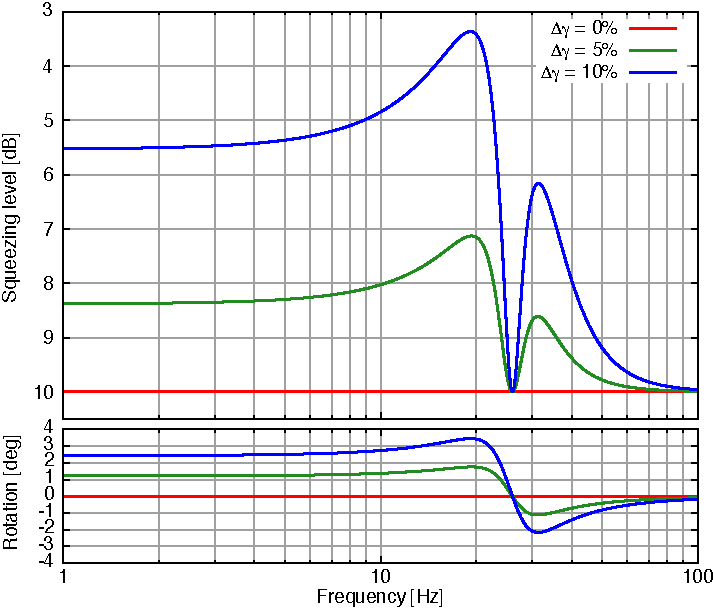
\includegraphics{./Sec_Optics/FCs-devbw-10-20-rotAI.pdf}
\caption{The figure illustrates the effect of a deviation of the required bandwidth. The lower graph shows the resulting residual phase-space rotation of the squeezing ellipse, the upper graph the according squeezing levels. Please note that the filter cavities are assumed to be lossless. Thus, the degradation of the squeezing level can be clearly traced back to the residual phase-space rotation.}
\label{fig:devBWll}
\end{figure}

Fig.~\ref{fig:devBW} shows the performance of the filter cavities (FC$_1$ and FC$_2$)  required for the ET- LF detector. Their bandwidth was varied according to a deviation of 1\,\% to 5\,\% from the designed value. In these plots, the round-trip loss of the filter cavities was considered to be 75\,ppm.

\begin{figure}
\centering
\includegraphics{./Sec_Optics/FCi-devbw_reviewAI.pdf}
\caption{The figure shows the squeezing spectra for a deviation of the designed bandwidth of a) the single FC$_1$  and b) the single FC$_2$. Graph c) shows the spectra if both  filter cavities are considered. In all cases, the filter cavity round-trip loss was considered to be 75\,ppm.}
\label{fig:devBW}
\end{figure}

If a tolerable  degradation  of the squeezing  by less than 2\,dB (related to the squeezing levels  achievable with  the  design parameters) is targeted, a deviation of the bandwidth less than 5\,\% is acceptable. From this value, the tolerances for the design parameters can be deduced. %They are listed in Tab. (XXX)

%Place tab here...

\FloatBarrier
\begin{figure}[htb]
\centering
\includegraphics[width=0.5\textwidth]{./Sec_Optics/cavity-designs.pdf}
\caption{Four geometries were analysed from the scattering point of view.}
\label{fig:sc_geometry}
\end{figure}
\paragraph{Choosing the optical layout of the filter cavity}\label{subsec:fcscattering}

%\emph{Author(s): K. Kokeyama, A. Freise, H. L{\"u}ck}

The Einstein Telescope required two 10\,km long and one comparatively
short (several hundred meters long) filter cavities per detector. 
Such filter cavities provide the correct frequency dependence for the injected squeezing state
in order to obtain broad band quantum noise suppression in the main interferometer.
The light reflected off these cavities needs to be injected into the
interferometer dark ports. In principle any cavity geometry can 
provide the correct filtering, however, practical concerns will 
put constraints on the geometry. %In this section we briefly discuss
%these issues, while a selection of the cavity geometry has not been done at this stage.
The four cavity geometries depicted in Fig.~\ref{fig:sc_geometry} are
possible candidates;
the following advantages and disadvantages follow directly from the
geometry (given a long baseline):
\begin{itemize} 
\item the 2-mirror cavity has the advantage of using only two mirrors but
  in order to extract the reflected beam, polarising optics are
  required which introduce additional optical losses and phase noise
\item the 3-mirror cavity provides the reflected beam without the need
  for extra optics. However, the small angle between the beams at the
  far right mirror means that the setup is more sensitive to small
  angle scattering, a problem which has been seen for example in the
  triangular input mode cleaner cavity of VIRGO. Another problem is
  that the large angle of incidence on the two left mirrors requires
  the mirrors to be significant larger compared to the 2-mirror setup.
  of the 10\,km long linear arm cavities. Since the ET optical design is 
  assuming the largest available mirrors being used for the linear arm cavity, this filter
  cavity geometry can be excluded. 
\item the rectangular 4-mirror setup also has the problem of requiring
  larger mirrors due to the angle of incidence.
\item The bow-tie cavity can separate the reflected beam from the
  injected one and does not feature large angles of
  incidence so that the mirror sizes are similar to those of a linear cavity. However, it 
  is sensitive to small angle scattering.
\end{itemize}

% motivation

A detailed study of scattering in the main interferometer and the
filter cavities has not been done yet. 
In Appendix~\ref{app:scatter} we provide a first analysis of the
amount of scattering between the suspended optics itself and conclude
that this effect can be ignored in the selection of the cavity geometry. 






% memo
% mirror surface and scattering
% BRDF
% 4 topologies were compared
% you have to be careful for the rectangular cavity due to the diagonal path
% possible scattering path such as direct back scattering, the effect
% baffles
% two mirror cavity's back scattering? 
\FloatBarrier
\subsubsection{Noise couplings}\label{sec:noise}
%We should consider\dots
%\begin{itemize}
%\item{Frequency noise}
%\item{Phase noise due to displacement noise}
%\item{Length stabilization}
%\item{Alignment noise/pointing?}
%\item{Scattering}
%\end{itemize}

In this section several noise mechanisms that potentially limit the detected squeezing levels are discussed. First, we discuss the effect of phase noise in the squeezing path. Assuming a self-homodyning
readout (DC readout) of the interferometers  signal field, the DC part of the interferometer output field serves as local oscillator. The quadrature of the signal field that is read out is determined by its relative phase with regard to this local oscillator. In order to reduce the quantum noise of this measurement, the relative phase of the injected squeezed field needs to be chosen such that the squeezed quadrature coincides with the readout quadrature. This required phase relation gets disturbed due to e.g.\ vibrating optical components in the squeezing path (displacement noise) or residual high frequency phase modulations that probably will be required for control purposes.  If the measurement time is greater than the period of the phase jitter period, the homodyne read out is not a pure measurement of a certain quadrature   $\Phi$ (e.g.\ the squeezed quadrature) but the integral over some span of $\Phi+\delta \Phi$. In this case, a certain fraction of the noise in the anti-squeezed quadrature is mixed into the measurement that was intended to be a measurement of the squeezed quadrature. It is obvious, that such a \textit{phase diffused squeezed state}  results in a degraded squeezing level.  Accordingly, an upper limit for the overall tolerable phase noise in the squeezing path needs to be deduced with regard to the targeted quantum noise reduction of 10\,dB.

The influence of phase noise on the squeezed field can be nicely illustrated by the accordant Wigner functions. We start from the Wigner function of a squeezed state that has a certain orientation (determined by the quadrature angle  $\varphi$) in phase-space. It is  given by
\begin{equation}
W(X_{1,\varphi},X_{2,\varphi}, \varphi) = \frac{1}{2\pi\sqrt{V_sV_a}}\exp\left[-\frac{X_{1,\varphi}^2}{2V_s}-\frac{X_{2,\varphi}^2}{2V_a}\right]\,.
\end{equation}
Here $V_s$ and $V_a$ denotes the variances in the squeezed and anti-squeezed quadrature, respectively (e.g.\ for a pure 10\,dB squeezed state  $V_s=0.1$ and $V_a=10$ if normalised to the variance of the vacuum state $V_{\rm{vac}}=1$).  The orientation in phase-space is accounted for by setting
\begin{eqnarray}
X_{1,\varphi} &=& X_1\cos(\varphi) - X_2\sin(\varphi)\\
X_{2,\varphi}  &= &X_1\sin(\varphi) + X_2\cos(\varphi)\,.
\end{eqnarray}
Here, the local oscillator serves as reference for the phase-space with its amplitude ($X_1$) and phase quadrature ($X_2$). The corresponding probability distribution in the amplitude quadrature ($X_1$) can be obtained from the Wigner function by integrating over $X_2$. One obtains
\begin{eqnarray}
P_{X_1} &=& \int\limits_ {-\infty}^{\infty}W_d(X_1,X_2)dX_2\\
&=&\frac{1}{{\sqrt{2\pi V_{X_1}(\varphi)}}}\exp\left[-\frac{X_1^2}{2V_{X_1}(\varphi)} \right]\,.
\end{eqnarray}
with the variance of the amplitude quadrature
\begin{eqnarray}
V_{X_1}(\varphi) &=& V_s\cos^2(\varphi) + V_a\sin^2(\varphi)\\
&=&\frac{1}{2}\left[V_s+V_a+(V_s-V_a)\cos(2\varphi)\right]\,.
\end{eqnarray}
Now, to describe a phase-diffused squeezed state, the quadrature angle $\varphi$ needs to be replaced by a probability density for the phase denoted as $\Phi(\varphi)$. Then, the Wigner function is given by
\begin{equation}
W_d(X_1,X_2) =\int \Phi(\varphi) W_d(X_1,X_2, \varphi)d\varphi\,.
\end{equation}
Again, the corresponding probability distribution in the amplitude quadrature ($X_1$) can be obtained from the Wigner function by integrating over $X_2$
\begin{equation}
P_{X_1,d} = \int\limits_ {-\infty}^{\infty}W_d(X_1,X_2)dX_2 \,.
\end{equation}
Accordingly, the variance of a phase-diffused squeezed state is given by
\begin{equation}
V_{X_1,d} = \int\limits_{-\infty}^{\infty}\Phi(\varphi)V_{X_1}d\varphi\,\Leftrightarrow  \int\limits_{-\infty}^{\infty}P_{X_1,d}X_1^2dX_1\,.\label{eq:varsqzphsdiff}
\end{equation}

\begin{figure}
\centering
\includegraphics[scale=0.77]{./Sec_Optics/Wig_10dB_all.jpg}
\caption{Illustration of the influence of a Gaussian distributed phase noise on the squeezed state. \textbf{Top:} Wigner functions for phase noise  with a standard deviation $\sigma$ of 0, 0.3, 0.6, 0.9. The initial, pure squeezed state was assumed with 10\,dB. \textbf{Bottom:} The probability distribution of the phase diffused squeezed states and the corresponding squeezing levels (red curves and red labels, respectively) in the  amplitude quadrature ($X_1$).  For comparison, the distribution of a vacuum state is shown (grey curves).}
\label{fig:phasediffusedSQZ}
\end{figure}

In Fig.~\ref{fig:phasediffusedSQZ} four Wigner functions  (top) and the corresponding probability distribution in the $X_1$-quadrature (bottom) are shown. We assumed a Gaussian-distributed phase noise, i.e,
\begin{equation}
\Phi(\varphi) = \frac{1}{\sqrt{2\pi\sigma^2}} \exp\left(-\frac{\phi^2}{2\sigma^2}\right)\,.
\end{equation}
We have considered phase noise with  a standard deviation $\sigma$ of 0 (no phase noise), 0.3, 0.6 and 0.9 (from left to right in Fig.~\ref{fig:phasediffusedSQZ}). The initial squeezed state (left figures) was assumed with $V_s=0.1$ and $V_a=10$, i.e.\ as a pure 10\,dB squeezed state. The degradation of the squeezing level due to phase noise becomes obvious from the comparison with the probability distribution of a vacuum state (grey traces in the bottom graphs). The probability distributions are labelled with the corresponding squeezing level. For strong phase noise  the initial squeezing is destroyed and the noise in the amplitude quadrature is even enhanced when compared to the vacuum noise (shot noise).

\begin{figure}
\centering
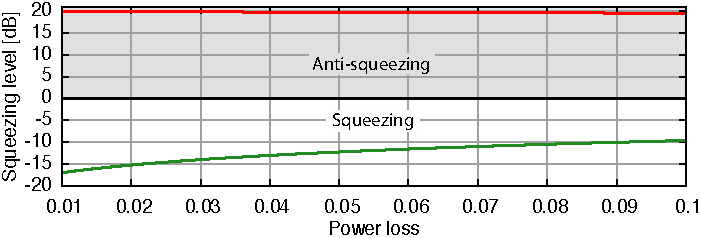
\includegraphics[scale=1]{./Sec_Optics/SQZ-20dB-losschartAI.pdf}
\caption{The degradation of the squeezing and anti-squeezing levels due to optical loss for an initially pure (no loss) 20\,dB squeezed state.}
\label{fig:20dBlosschart}
\end{figure}

The illustration in Fig.~\ref{fig:phasediffusedSQZ} implies that the larger the anti-squeezing level, the larger the effect of phase noise. In fact, in order to achieve the targeted quantum noise reduction of 10\,dB, a squeezed light source needs to be utilised that generates considerably more than 10\,dB (anti-)squeezing to compensate for possible loss. If an overall optical loss of up to 10\,\% in the squeezing path (including 1\,\% loss in the squeezed light source itself) is assumed, an initially pure 20\,dB squeezed state needs to be generated. The degradation of the squeezing (and anti-squeezing) level with optical loss is shown in Fig.~\ref{fig:20dBlosschart}. Whereas the squeezing level is strongly affected by optical loss, the anti-squeezing level is not considerably reduced. Considering an overall optical loss of 10\,\% the squeezing level is reduced from 20\,dB to about 9.6\,dB, but the anti-squeezing level is still about 19.5\,dB. In Fig.~\ref{fig:phasediffusedSQZ20dB} the effect of phase noise on an initial 20\,dB squeezed state is illustrated, for which optical loss of 1\,\%, 3\,\%, 5\,\% and 10\,\% was considered. Here the phase noise was assumed with a standard deviation of $\sigma=0.3$. Again,  the top graphs show the Wigner functions and the bottom graphs the probability distribution in the amplitude quadrature. Here, in each case three traces are plotted. The red trace is the distribution of the phase diffused squeezed state and the black one that of a vacuum state. The grey curves correspond to the distribution without phase noise, i.e.\ the degradation of the squeezing level only due to the considered optical loss can be deduced. Again, it can be seen that the high phase noise destroys the squeezing. In each case, the resulting noise level is considerably enhanced when compared to the shot noise level. Please note that although the squeezing levels in the undisturbed case are $\geq$10\,dB, the high anti-squeezing level of almost 20\,dB leeds to higher noise levels when compared to the pure 10\,dB squeezed state (refer to Fig.~\ref{fig:phasediffusedSQZ}). I.e.\ in presence of phase noise the achievable squeezing level can be  optimized by reducing the anti-squeezing (and thus the squeezing) generated by the squeezed light source. On the other hand, that means that in presence of considerable phase noise a compensation of optical loss in the  squeezing path is not possible by enhancing the  squeezing (and thus the anti-squeezing) generated in the squeezed light source.

\begin{figure}
\centering
\includegraphics[scale=0.77]{./Sec_Optics/Wig_20dB_loss.jpg}
\caption{Degradation of a pure 20\,dB squeezed state due to optical loss and phase noise.}
\label{fig:phasediffusedSQZ20dB}
\end{figure}


In the previous investigation comparatively high values for the phase noise was considered for illustration purpuses. Such high values are not expected to be present in a realistic experimental environment. However, the upper limit for the overall phase noise in the squeezing path depends on the squeezed state, that is generated by the squeezed light source. Table~\ref{tab:phsnoiselimit} lists the allowed phase noise (i.e.\ its standard deviation) for several conditioned squeezed states. The states were constituted for several values of the optical power  loss $l^2$ such that the  squeezing level without phase noise is 10\,dB. The required squeezing  that needs to be generated inside the squeezed light source can be calculated according to
\begin{equation}
V_s = 0.1 -l^2\hspace{11pt}\text{and}\hspace{11pt}V_a = \frac{1}{V_s}.
\end{equation}
We relates the upper limit $\sigma_{\rm max}$ for the phase noise to a squeezing level that is reduced to 9\,dB due to the phase noise. As the phase noise is assumed to be Gaussian-distributed with zero mean, Eq.~(\ref{eq:varsqzphsdiff}) can be solved giving
\begin{equation}
V_{X_1,d} = \frac{1}{2}\left[V_s+V_a+(V_s-V_a)\exp\left(-2\sigma^2\right)\right]\,.\label{eq:varianzsqzpn}
\end{equation}
Soving Eq.~(\ref{eq:varianzsqzpn}) for $\sigma$ yields
\begin{equation}
\sigma = \sqrt{-\frac{1}{2}\log\left[\frac{2V_{X_1,d}-V_s-V_a}{V_s-V_a}\right]}\,.
\end{equation}
From this equation the tolerable phase noise characterised  by $\sigma_{max}$ can be calculated for the targeted variance  $V_{X_1,d}=0.1$ and squeezing level of 10\,dB, respectively.


\begin{table}[h]
\begin{center}
\begin{tabular}{rrrrr}
\hline
\hline
optical loss [\%]& initial squeezing [dB] & squeezing [dB] & anti-squeezing [dB] & $\sigma_{\rm max}$ \\
\hline
1 & -10.41 & -10 & 10.37 & 0.049\\
3 & -11.41 & -10 & 11.29 & 0.044\\
5 & -12.79 & -10 & 12.58 & 0.038\\
9 & -19.59 & -10 & 19.19& 0.018 \\
10 & $-\infty$ & -10 & $\infty$ & 0\\
20 & $-\infty$ & -6.99 & $\infty$ & 0\\
\hline
\hline
\end{tabular}
\end{center}
\caption{The table lists  the squeezing and anti-squeezing levels and the tolerable phase noise for several values of optical loss.}
\label{tab:phsnoiselimit}
\end{table}

From the tolerable $\sigma_{\rm max}$ we will deduce in following investigations
\begin{itemize}
\item{the allowed displacement noise in the  filter cavities}
\item{the requirements for the filter cavity length stabilization}
\item{the requirements on frequency noise of the squeezed light source related to main interferometer beam}
%\item{Alignment noise/pointing?}
%\item{Scattering}
\end{itemize}
\FloatBarrier
\subsubsection{Length control of the filter cavities}
We will analyse
\begin{itemize}
\item{the realisation of a locking scheme without introducing too much optical loss (due to pick-off mirrors needed for detection ports). }
\item{the potential of using the orthogonal polarisation for error signal generation.}
\item{the restrictions to RF sidebands. They need to be in the same mode as the squeezing, therefore generated in the squeezer by means of the coherent control beam.}
%\item{RF Frequencies. Needs to be reflected at least at the OMC in order not to spoil the IFO.}
\item{A ring -vs- a linear filter cavity design. If linear filter cavities are used additional Faraday rotators are required.}
%\item{Put the above just as note at a certain point, e.g. within the noise section}
\end{itemize}

